\documentclass[12pt]{article} 
\usepackage[left=2cm, right=2cm, top=2cm, bottom= 2cm]{geometry} 
\usepackage{graphicx,epsfig,verbatim,enumerate}
\usepackage{amssymb,amsmath,amsthm,amsbsy}
\usepackage{ifthen}
\usepackage{morefloats}
\usepackage[hidelinks]{hyperref}
%\hypersetup{colorlinks=true, linkcolor=blue}
\usepackage{cite}
\usepackage{color}
\usepackage{textcomp}
\usepackage{float}

\newcommand{\todo}[1]{\noindent\textcolor{blue}{{$\Box$ #1}}}

\title{Mixed and Pure Breed Dog Classifier}
\date{\today}
\author{Luke Trinity and Nat Shenton \\ CS 254}

\begin{document} 
\maketitle
\section{Introduction}

Online sources of high resolution images including Google, Image-net \cite{deng2009imagenet}, and Flickr are providing new opportunities to explore applications of image categorization using computer vision. One interesting application in the field of fine-grained image classification is identification of dog breed. Dogs faces are considered to be highly differentiable for each breed, which makes classification an approachable problem. However, the work is challenging due to the varying combinations of facial characteristics and color patterns between species, as well as intra-class variation within a single species. Another aspect of the problem that makes it more complicated is the presence of humans and man-made backgrounds, which are not as common in other animal datasets. In addition, many attempts to classify dog breeds fail to corroborate the results with actual DNA evidence. Our approach will be to utilize an existing dog breed image classification dataset \cite{khosla2011novel}, in combination with a novel dataset that includes paired DNA test results and photos \cite{voith2009comparison} and crowd sourced mixed breed dog images, to classify dogs as pure bred or mixed breed. 

\section{Problem Definition and Algorithm}

\subsection{Task Definition}

The task is to take dog images where each image is labeled either mixed or pure breed and use them to train an algorithm to classify an unseen photo based on whether the dog is mixed or pure. An important part of training our neural network is to normalize the input images. Each input image is defined as a matrix of $250\times 250\times3$. The output of this algorithm will either be a mixed or pure bred dog. Potential benefits of this work are to provide dog owners an easy way to classify if their dog is a pure bred or mixed, or assist shelters in generating interest in dogs to increase adoption rates. From a machine learning perspective, our testing suite produces interesting and thought provoking results about how to select a model in a difficult decision space. It could be an exciting way to start a conversation and help people learn about different breeds of dogs, and how they are mixed. The final goal for this task would allow for a dog owner to upload a picture of their dog to a website or app and then the machine learning algorithm will classify their dog as the pure bred breed or the top two possible breeds.

\subsection{Dataset}

The Stanford Dogs Dataset has 20,580 images each classified into one of 120 classes of dog breed. \cite{khosla2011novel} Each image also has an associated bounding box identifying the location of the dog within the photo. The mixed-breed DNA identified dog photo dataset from Voith et al. \cite{voith2009comparison} has 20 images, each paired with DNA percentage breakdown of dog breed. The final mixed breed data used crowdsourcing to bring the total up to 266 pictures. There was no way to actually identify if the dog was actually mixed or not so we are assuming that the submission of the mixed breed dog is correct in the data. The final dataset was obtained by a random sampling of pure bred dogs from the Standard dataset equal to the length of the amount of dogs form the Stanford Dogs Dataset, giving us a balanced dataset of 532 images. 

\subsection{Algorithm Definition}

First, we utilize the Resnet50 convolutional neural network \cite{he2015deep} as it achieves roughly 80\% accuracy on the Standford dog dataset in classifying pure bred dogs. This pretrained neural network gives a classification accuracy high enough that it should classify an image of a purebred dog correctly. The convolutional neural network is trained on Google's ImageNet which contains the Stanford Dogs dataset. By feeding images from the mixed dog breed dataset into this pretrained neural network, the network gives the output as the probability of each dog breed. The output from Resnet50 contains the probabilities of 1000 labels, and our algorithm used the top 4 highest probabilities. From here principal component analysis is used to take the four prediction outputs from the pretrained convolutional neural network down to two features. With these two features as the input classes, a sweep of four classification methods were used: linear kernel SVM, optimal kernel SVM, random forest, and a neural network.

\begin{figure}[H]
\centering{
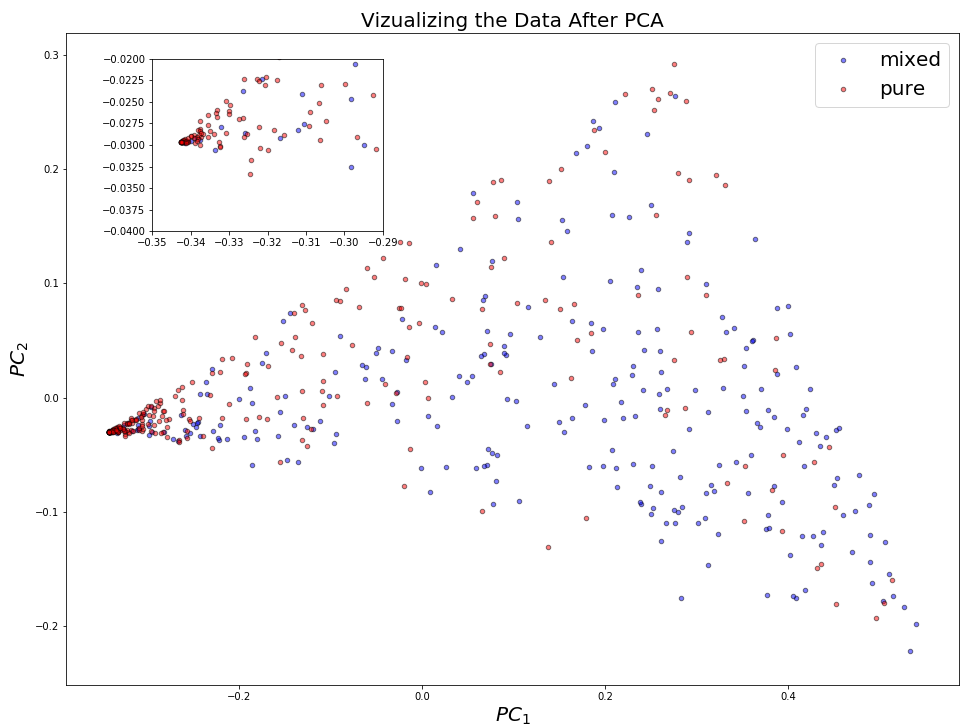
\includegraphics[width=0.7\textwidth]{Data_vis}
}
\caption{The distribution of the data after using principal component analysis to reduce the breed probabilities from 4 features to 2. Red is purebred while blue is mixed. The inset plot shows the area where the data in clustered.}
\end{figure}

\section{Experimental Evaluation}

\subsection{Methodology}

For the SVM linear kernel we used cross validation to search over C values randomly drawn from an exponential distribution (scale=1000), $\gamma$ values randomized over an exponential distribution (scale = 2), and randomly choosing between balanced or no class weight. For the SVM optimal kernel, the cross validation search over Radial Basis Function kernel and polynomial kernel. The random forest algorithm looks at a forest of 30 trees, and draws randomly from a uniform distribution for the minimum number of samples to split on as fraction of the total number of samples. For random forest we also randomly validated for a max depth as a random integer between 1 and 50. Before moving on to neural network testing suite description, please note that for the cross validation specified above, 15 fold was used across model types, and the randomized search cross validation searched over 200 iterations for each model.

\begin{figure}[H]
\centering{
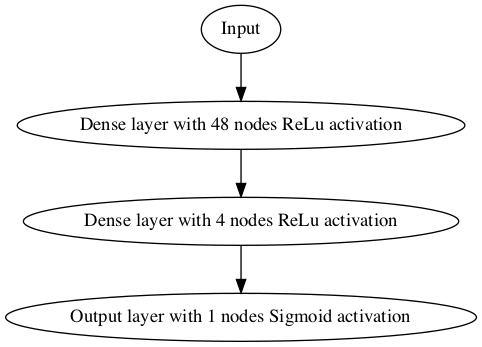
\includegraphics[width=0.5\textwidth]{nueral_netgv}
}
\caption{Neural Network Structure}
\end{figure}

The neural network uses an architecture of 3 hidden fully connected layers with the ReLu activation function. The first layer contains 48 nodes, the second 24 nodes, and the third 4 nodes; each with bias and kernel constraints. The output layer contains one node with a sigmoid activation function. The model was then compiled with the Adam gradient descent optimizer, and binary cross-entropy as the loss function. The neural network was trained over 300 epochs. For each of the four model types described, we trained as described above, and tested 250 different splits of the data with a 66-33 training testing split. Here we report the accuracy, as well as the different between the training and test accuracy, for each of those 1000 models grouped by model type.

\begin{figure}[H]
\centering{
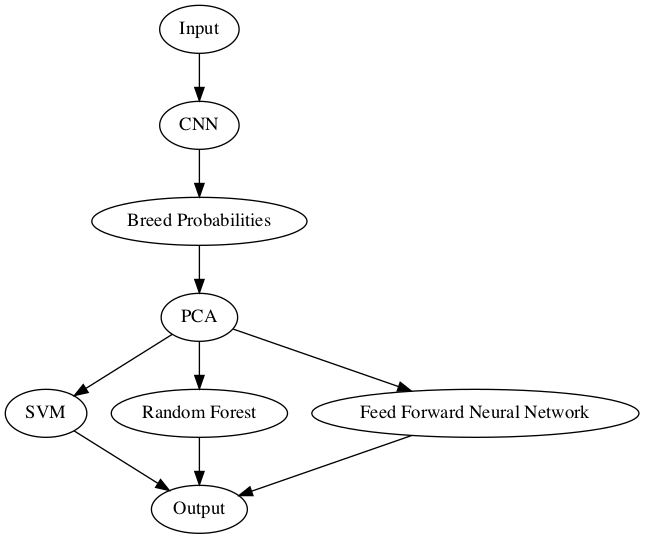
\includegraphics[width=0.5\textwidth]{modelgv}
}
\caption{Model Testing Suite Visualization}
\end{figure}

\subsection{Additional Neural Network Methodology}

In the results section we present the conclusion that neural networks are performing the best on our dataset. To further test how different neural network architectures might affect accuracy, we increased and decreased the number of nodes in our hidden layers and ran a similar experiment. This second testing suite is used to test the three neural network architectures to increase performance. In addition to our initial neural network (48, 24, 4, and 1 nodes in each hidden layer) which we will refer to as `medium’ depth, we also test a `less deep’ model (24, 12, 2, and 1 nodes in each hidden layer) and a deeper model (96, 48, 8, 1 nodes in each hidden layer). The same bias and kernel constraints were used for each of the neural networks, which were trained for 300 epochs each on the same 250 splits on the data. For these 750 total models tested, we again report the accuracy and training-test accuracy distributions.

\subsection{Results}

Here are the results of the initial testing suite. Figure 4 shows the distribution of accuracy scores. Here this shows the initial testing suite results with each model run 250 times. The SVM are using random search cross validation what the only parameters changed in the testing. 

\begin{figure}[H]
\centering
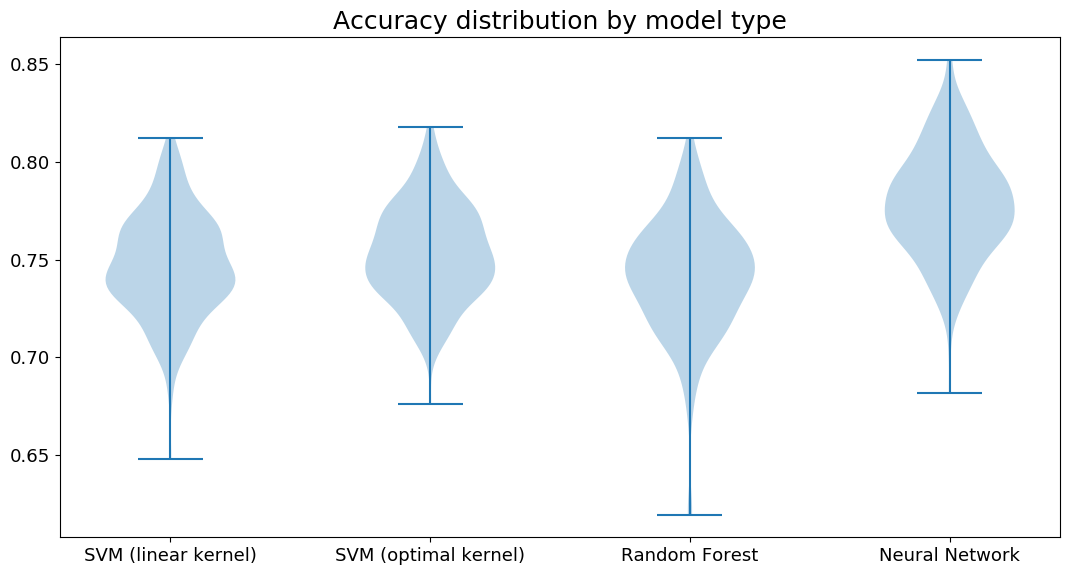
\includegraphics[width=0.7\textwidth]{testOut}
\caption{The violin plot shows the distribution of testing accuracy of each model type from the testing sweep.}
\end{figure}
Figure 4 shows that SVM with linear kernel, SVM with a non-linear kernel, and random forests perform about the same, but the neural network with the architecture shown in figure 1 gives the best accuracy. The table gives the numeric results of this suite.

\begin{table}[H]
\centering
\begin{tabular}{l|l|l}
\hline
\multicolumn{1}{|l|}{Model Type} & Mean  & \multicolumn{1}{l|}{Standard Deviation} \\ \hline
SVM (linear kernel)              & 0.747 & 0.026                                   \\
SVM (optimal kernel)             & 0.753 & 0.024                                   \\
Random Forest                    & 0.742 & 0.030                                   \\
Multi Layer Perceptron           & 0.780 & 0.028                                  
\end{tabular}
\end{table}
Figure 5 gives the $\text{Accuracy}_{\text{Testing}} - \text{Accuracy}_{\text{Training}}$ for each model. This gives a representation of the overfitting and under-fitting the models could be experiencing. Here it seems that the neural network is overfitting the data with the mostly negative values.
\begin{figure}[H]
\centering
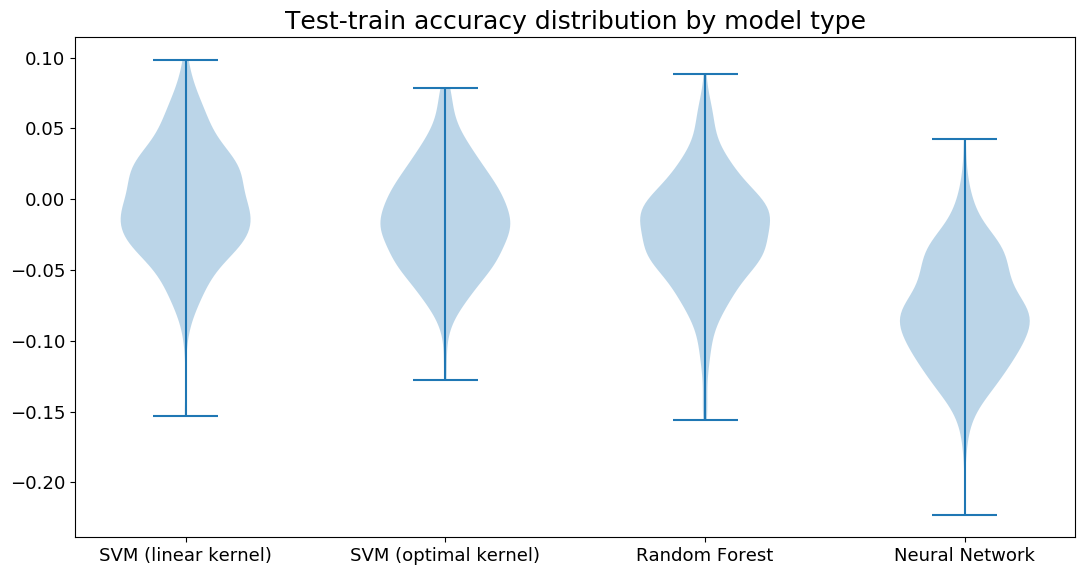
\includegraphics[width=0.7\textwidth]{testOut2}
\caption{The violin plot shows the distribution of the $\text{Accuracy}_{\text{Testing}} - \text{Accuracy}_{\text{Training}}$
for each model. }
\end{figure}
The numeric results of the different between the testing and training is found in the table below.

\begin{table}[H]
\centering
\begin{tabular}{l|l|l}
\hline
\multicolumn{1}{|l|}{Model Type} & Mean   & \multicolumn{1}{l|}{Standard Deviation} \\ \hline
SVM (linear kernel)              & -0.003 & 0.039                                   \\
SVM (optimal kernel)             & -0.014 & 0.036                                   \\
Random Forest                    & -0.022 & 0.039                                   \\
Multi Layer Perceptron           & -0.080 & 0.039                                  
\end{tabular}
\end{table}

The decision boundary of the used in first testing suite neural network is found in figure 6. 
\begin{figure}[H]
\centering
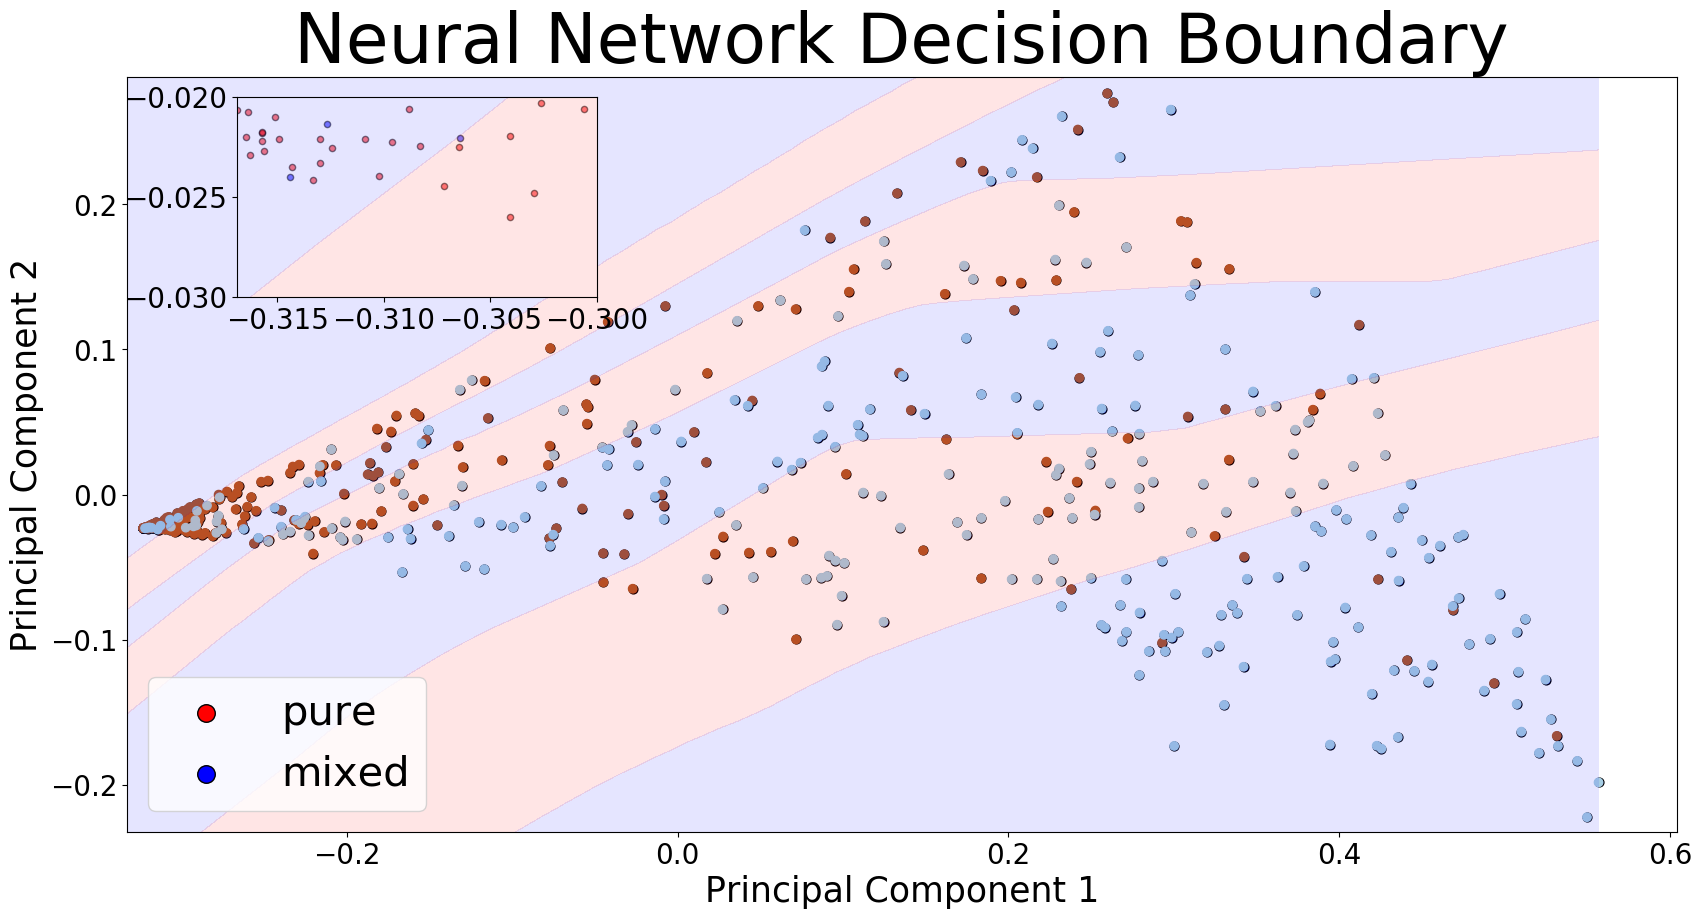
\includegraphics[width=0.7\textwidth]{decboundary}
\caption{The decision boundary of the neural network shown in figure 1.}
\end{figure}
The results of the neural network testing suite are shown in figure 7. 
\begin{figure}[H]
\centering
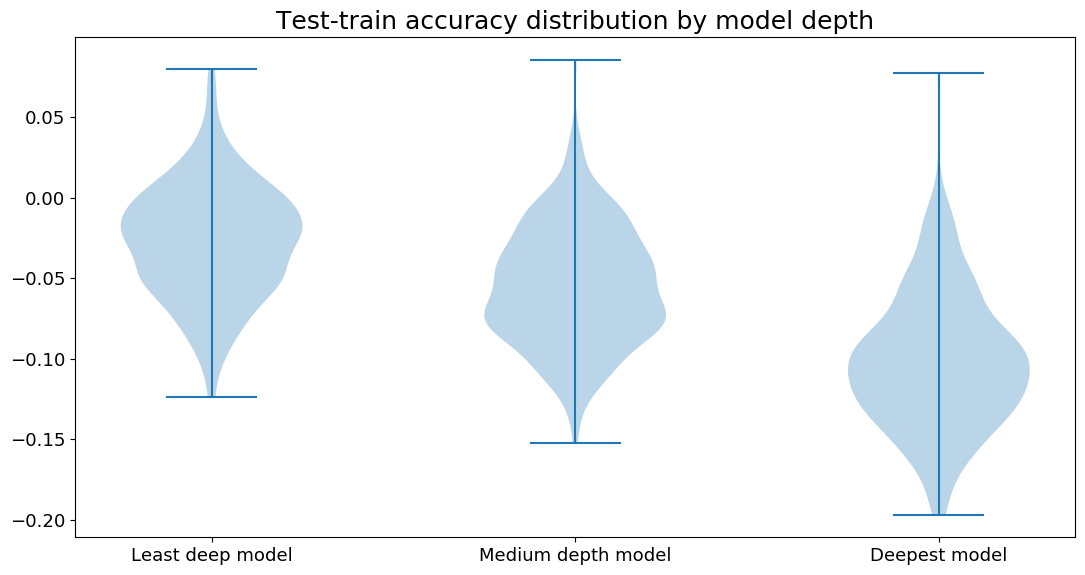
\includegraphics[width=0.7\textwidth]{testOut1289}
\caption{The violin plot shows the distribution of testing accuracy of each neural network type from the testing sweep.}
\end{figure}
The numeric results of the testing suite are found in the table below.  

\begin{table}[H]
\centering
\begin{tabular}{l|l|l}
\hline
\multicolumn{1}{|l|}{Model Type}                                   & Mean   & \multicolumn{1}{l|}{Standard Deviation} \\ \hline
Least Deep (24-\textgreater{}12-\textgreater{}2-\textgreater{}1)   & 0.7899 & 0.027                                   \\
Medium Depth (48-\textgreater{}24-\textgreater{}4-\textgreater{}1) & 0.7863 & 0.025                                   \\
Deepest (96-\textgreater{}48-\textgreater{}8-\textgreater{}1)      & 0.7966 & 0.030                                  
\end{tabular}
\end{table}

Figure 8 gives the $\text{Accuracy}_{\text{Testing}} - \text{Accuracy}_{\text{Training}}$ of each neural network. 
\begin{figure}[H]
\centering
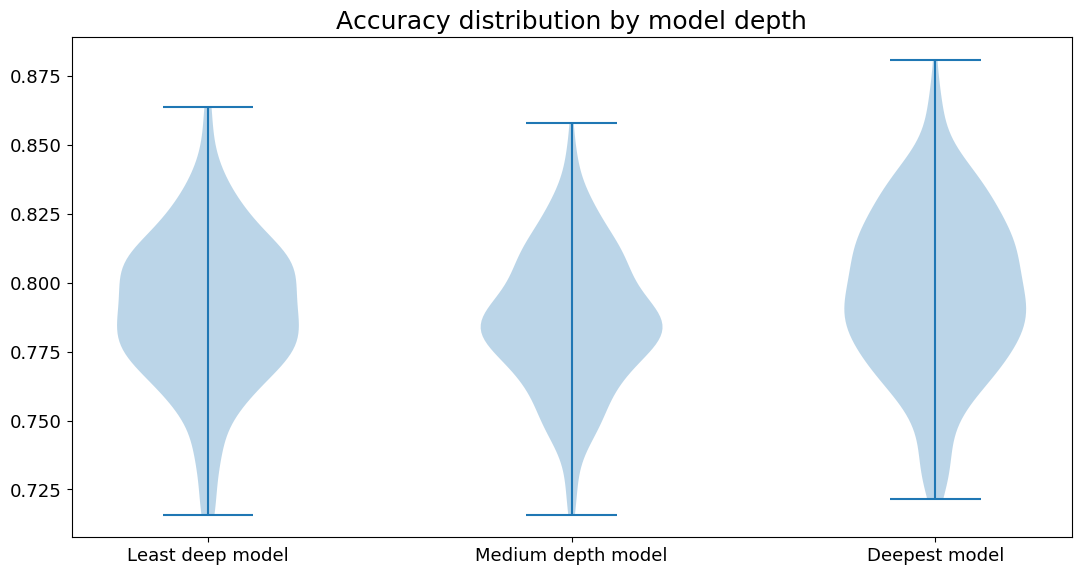
\includegraphics[width=0.7\textwidth]{testOut128}
\caption{The violin plot shows the distribution of the $\text{Accuracy}_{\text{Testing}} - \text{Accuracy}_{\text{Training}}$
for each neural network. }
\end{figure}

The numeric results of figure 8 are shown in the table below.

\begin{table}[H]
\centering
\begin{tabular}{l|l|l}
\hline
\multicolumn{1}{|l|}{Model Type}                                   & Mean   & \multicolumn{1}{l|}{Standard Deviation} \\ \hline
Least Deep (24-\textgreater{}12-\textgreater{}2-\textgreater{}1)   & -0.027 & 0.035                                   \\
Medium Depth (48-\textgreater{}24-\textgreater{}4-\textgreater{}1) & -0.055 & 0.037                                   \\
Deepest (96-\textgreater{}48-\textgreater{}8-\textgreater{}1)      & -0.102 & 0.042                                  
\end{tabular}
\end{table}

\subsection{Discussion}

From the testing suite, the neural network algorithm above shows that the 

\section{Related Work}

In the initial article utilizing the novel dataset by Khosla et al. \cite{khosla2011novel}, the mean accuracy reached 22\% when 100 training images were utilized within the SIFT methodology. Liu et al. \cite{liu2012dog} reached 69\% accuracy, with greater success than Khosla et al. \cite{khosla2011novel} due to their partially localized approach. We hope to leverage the bounding boxes and augment the work of Liu et al. \cite{liu2012dog}, possibly improving on their methodology to achieve higher accuracy. Several bounding box approaches are currently being reviewed, although all are endlessly modifiable from simple image segmentation. One is a slight adaptation to a method often employed for training algorithms to images of different shade and dimension called DeepCut. \cite{rajchl2016deepcut} There are several standard variations on the basic DeepCut methodology, which hones in on the nature and dimension of the bounding in a cookie-cutter, traced-out way as opposed to any kind of geometric shape. There was also a Kaggle competition to create the best dog breed classifier of 16 breeds sampled from the Stanford Dog dataset. Here competitors use transfer learning to create the best breed classifier. Competitors were able to get classification scores above 95\% in this competition \cite{kaggledogs}. Microsoft has a dog classifier built on their Bing platform. This platform was used as inspiration for the web app.

%A very similar methodology is known as GrabCut which does not need to even be a single, continuous cookie-cutter-style line bounded around a desired segment of an image. GrabCut is standardly designed to grab multiple disparate segments of an image at once for a single, desired analysis. In addition to one of these approaches or some modification thereof, we plan to incorporate some aspect of KL Loss to account for localization uncertainty which could greatly assist with interference from background objects such as people, buildings, trees, etc. \cite{he2019bounding} There are, of course, a number of other modifiable ‘standard’ or ‘familiar’ combinations of approaches to deal with bounding and uncertainty to also be explored. Even so, most will lead to an approximately similar result if implemented correctly. Deep/GrabCut is simple and can narrow the selected image segment in a convenient, efficient manner. KL Loss will be further researched and incorporated to deal with expected shading difficulties, image blurring and background/foreground image ‘noise’.

%talk about Kaggle Compitetion

%\section{Next Steps}

%The initial Neural network trained using Keras shows the classification of dog breeds gets worse and worse as more breeds are introduced. From these results there are two main directions this project will have to go. The first is it move this project onto the VACC, which should avoid the memory error when running any more than a 7 breed classification which occurred on the local machine. We will test the performance of both the Bluemoon and DeepGreen supercomputer clusters to scale the model from the 7 breed classification to the 120 breed classification. The model will return the prediction probability vector for all breeds. This will be Luke's main task.

%The second task will be to improve the model. Using cross validation, the pre-weighted neural networks from the Keras libraries will be used to improve the model. Keras has an extensive library of pre-weighted networks specifically designed from image classifications. This will include the tuning of hyper parameters to improve the prediction probability through cross validation, as well as going inside the black box that is the neural network and experimenting with different numbers and types of sequential layers. This will be Nat's main task. 

%Once the algorithm has been optimized, the final step of the project will be a user interface where a user will upload an image of their dog, and the algorithm will return the prediction probability. This will either be done with a simple HTML page or using the Unity platform. 

\section{Code and Dataset}

The code can be found in our github repo: \url{https://github.com/nshenton/CS_251_DogProject}. Please see the Readme in the repo for more information. The Stanford Dogs Dataset can be downloaded from this page: \url{http://vision.stanford.edu/aditya86/ImageNetDogs/}. Please contact the authors for the mixed dog dataset.

\section{Conclusion}

Here we have described our barebones methodology and presented intermediate results. Our path forward will involve a team effort of improving the accuracy of our model, and leveraging the technologies of the VACC. We believe our final product will be interesting and a great conversation starter for dog lovers and machine learning enthusiasts alike. Our elavator pitch is simple, wouldn't you like to upload a photo of your dog and see what breeds it could potentially be? Looking past this semester, it would be a long-term goal to incorporate user feedback into the training of the model, i.e. having users rate the predictions for how accurate they are perceived to be. 

\nocite{*}
\bibliography{dogbib}{}
\bibliographystyle{ieeetr}

\end{document}
